
\section{Бандиты}\label{sec:bandistssection}

\subsection{Задача многоруких бандитов}

Рассмотрим сильно упрощённую задачу RL, где эпизод заканчивается после первого шага.

\begin{example}
В игровом зале стоят в ряд $|\A|$ игровых автоматов (<<одноруких бандитов>>): в каждый можно отправить монетку, дёрнуть за ручку, и тогда автомат с некоторой вероятностью выдаст вам приз. Вероятность приза фиксирована для каждого автомата (зависит от настроек, выставленных владельцами зала...), но может различаться между автоматами. 

\needspace{5\baselineskip}
\begin{wrapfigure}{r}{0.25\textwidth}
\vspace{-0.6cm}
\centering
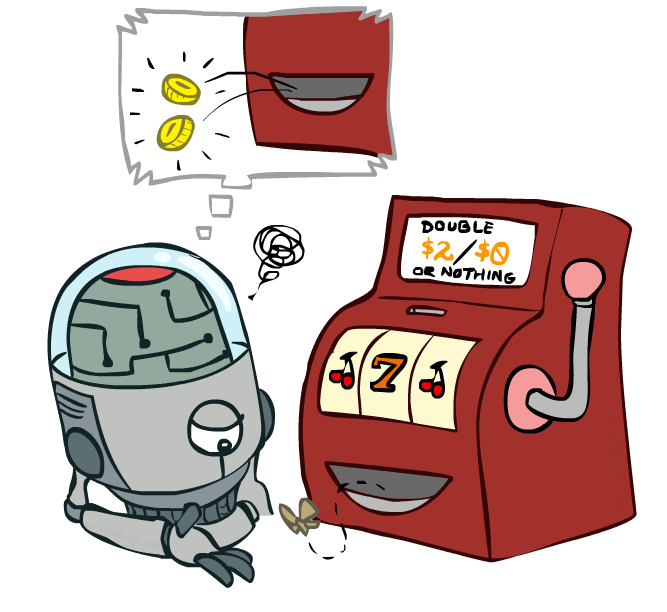
\includegraphics[width=0.25\textwidth]{Images/bandits.png}
\vspace{-0.3cm}
\end{wrapfigure}

Игроку (агенту) доступна только информация о том, получил ли он приз или нет, и всё, что он может --- это пробовать дёргать за ручки разных автоматов. Задача --- как можно быстрее выучить, какую ручку дёргать наиболее выгодно на основе накапливаемого опыта. Однако, без знания истинных вероятностей у игрока возникает вопрос: действительно ли тот автомат, который согласно его опыту выдавал приз чаще, является самым хорошим, или ему просто везло? Или с автоматом, который редко выдавал приз, просто было сыграно слишком мало игр? Налицо проблема exploration-exploitation дилеммы, которую в таком упрощённом виде легче теоретически анализировать.
\end{example}

Формально мы рассмотрим задачу RL для MDP, в котором нет состояний (<<есть только одно состояние>>). Агент выбирает действие при помощи стратегии $\pi(a)$ и получает какой-то приз из автомата с выбранным номером, после чего эпизод заканчивается. Формально мы будем интерпретировать это как стохастичную функцию награды, которая зависит только от выбранного игроком действия.

\begin{definition}
\emph{Многорукий бандит} (multi-armed bandit) --- это $A$ распределений на вещественной оси $p(r \mid a)$, $a \in \{1,2,3 \dots A\}$.
\end{definition}

Понятно, что в данной задаче Q-функция не зависит от стратегии и всегда равна
$$Q(a) = \E_{p(r \mid a)} r,$$
а оптимальная V-функция --- скаляр, равный Q-функции оптимального действия, <<наилучшего автомата>>:
$$V^* = \max\limits_a Q(a)$$

После каждого эпизода (т.е. после каждого шага) мы вольны улучшить свою стратегию, поэтому с каждым эпизодом наша стратегия меняется. Полный процесс, соответственно, задан следующим образом: на $k$-ом эпизоде мы сэмплируем $a_k \sim \pi_k(a)$ и наблюдаем награду $r_k \HM\sim p(r \HM\mid a_k)$, затем как-то меняем свою стратегию и получаем $\pi_{k+1}$. 

Допустим, всего проводится $T$ итераций обучения (играется $T$ эпизодов). Если бы мы знали оптимальную ручку, мы бы сыграли все $T$ эпизодов именно с ней, получив $TV^*$ награды. Но нам придётся сколько-то итераций потратить на поиск этой самой ручки --- на <<исследования>> --- и за счёт этого мы проиграем за каждое неоптимальное действие $a_k$ в среднем объёме $V^* \HM- Q(a_k)$.

\begin{definition}
\emph{Сожалением} (regret) за $T$ эпизодов называется величина
$$\Regret_T \coloneqq T V^* - \sum_{k=0}^T Q(a_k)$$
\end{definition}

Задача многорукого бандита --- поиск такой процедуры обучения $\pi$, которая минимизировала бы наши средние сожаления. В первую очередь здесь интересны асимптотически оптимальные стратегии с точки зрения сожалений: что $\lim\limits_{T \to \infty} \E \Regret_T$, где мат.ожидание берётся по $\pi_1, \pi_2 \dots$, ведёт себя в некотором смысле наилучшим возможным образом.

\subsection{Простое решение}

Единственный способ оценивать $Q(a)$ --- по Монте-Карло. На $k$-ом шаге мы можем оценить каждую Q-функцию как
$$Q_k(a) \coloneqq \frac{\sum_k r_k [a_k = a]}{\sum_k [a_k = a]}$$

Как мы обсуждали в разделе про экспоненциальное сглаживание, обновление такой Монте-Карло оценки $Q_k(a)$ через счётчики по сути и есть обучение: пусть $n_k(a)$ --- счётчик, сколько раз мы выбирали действие $a$ за все эпизоды, тогда:
\begin{align*}
Q_k(a_k) &= \left( 1 - \frac{1}{n_k(a_k)} \right)Q_{k-1}(a_k) + \frac{1}{n_k(a_k)} r_k = \\
&= Q_{k-1}(a_k) + \frac{1}{n_k(a_k)} \left( r_k - Q_{k-1}(a_k) \right)
\end{align*}

Весь вопрос заключается в том, как на основе этих оценок и знания, сколько раз какое действие было попробовано --- величины $n_k(a_k)$ --- выбирать действия. Понятно, что жадный выбор может завести нас в ситуацию, когда мы будем всё время играть с не самой оптимальной ручкой.

\begin{proposition}
При любом алгоритме скорость роста сожалений не более чем линейная: для некоторой константы $C$
$$\E \Regret_T \le CT$$
\begin{proof}
Рассмотрим худшую стратегию, которая всегда выбирает худшее действие с наибольшими сожалениями $\max\limits_a \left( V^* - Q(a) \right)$. Тогда сожаления за $T$ эпизодов будут равны
$$\Regret_T = T \max\limits_a \left( V^* - Q(a) \right)$$
Понятно, что это верхняя оценка на сожаления любого алгоритма, и $\max\limits_a \left( V^* - Q(a) \right)$ --- константа $C$ в линейной скорости роста.
\end{proof}
\end{proposition}

\begin{proposition}
При жадном выборе сожаления растут с линейной скоростью: для некоторой константы $C$
$$\E \Regret_T \ge CT$$
\begin{proof}
С некоторой вероятностью $\alpha$ жадный алгоритм застрянет на постоянном выборе автомата $a$ с ненулевым регретом $V^* - Q(a)$ и продолжит выбирать его до бесконечности. Тогда в среднем регрете появится слагаемое $T \alpha (V^* - Q(a))$, следовательно как минимум можно в качестве константы $C$ выбрать $\alpha (V^* - Q(a))$.
\end{proof}
\end{proposition}

Наивное решение --- решать проблему эксплорейшна при помощи $\eps$-жадной стратегии \ref{egreedy}.

\begin{algorithm}{Наивный бандит}
\textbf{Гиперпараметры:} $\eps(k)$ --- стратегия исследования

\vspace{0.3cm}
Инициализировать $Q_0(a)$ произвольно \\
Обнулить счётчики $n_0(a) \coloneqq 0$ \\
\textbf{На очередном шаге $k$:}
\begin{enumerate}
    \item выбрать $a_k$ случайно с вероятностью $\eps(k)$, иначе $a_k \coloneqq \argmax\limits_{a_k} Q_k(a_k)$
    \item увеличить счётчик $n_k(a) \coloneqq n_{k-1}(a) + [a_k = a]$
    \item пронаблюдать $r_k$
    \item обновить $Q_k(a) \coloneqq Q_{k-1}(a) + [a_k = a] \frac{1}{n_k(a)} \left( r_k - Q_{k-1}(a) \right)$
\end{enumerate}
\end{algorithm}

\begin{proposition}
При $\eps$-жадном выборе сожаления всё равно растут с линейной скоростью: для некоторой константы $C$
$$\E \Regret_T \ge CT$$
\begin{proof}
Поскольку на каждом шаге с вероятностью $\frac{\eps}{|\A|}$ мы выбираем некоторое неоптимальное действие $a$ с ненулевым регретом $V^* - Q(a)$, в среднем регрете появится слагаемое $T \frac{\eps}{|\A|} (V^* - Q(a))$, следовательно как минимум можно в качестве константы $C$ выбрать $\frac{\eps}{|\A|} (V^* - Q(a))$.
\end{proof}
\end{proposition}

\begin{remark}
В случае нестационарных бандитов распределения $p(r \HM\mid a)$ тоже меняются со временем и куда-то плывут. Наивное решение в такой ситуации можно модифицировать костыльми. Во-первых, $\eps$ нельзя уменьшать к нулю, необходимо постоянно пробовать различные действия, поэтому можно выставить $\eps$ в константу. Во-вторых, вместо счётчиков будем обновлять информацию о Q-функции через экспоненциальное сглаживание:
$$Q_k(a_k) = Q_{k-1}(a_k) + \alpha \left( r_k - Q_{k-1}(a_k) \right)$$
где $\alpha < 1$ --- константный гиперпараметр.
\end{remark}

\subsection{Теорема Лаи-Роббинса}

Можно ли придумать что-то лучшее, чем линейная скорость роста регрета? Перепишем регрет чуть-чуть по-другому:

\begin{proposition}
\begin{equation}\label{regretalt}
\Regret_T = \sum_{a} n_T(a) (V^* - Q(a))
\end{equation}
\end{proposition}

Понятно, что действия с большим регретом $V^* - Q(a_k)$ нужно выбирать как можно меньше, то есть асимптотически уменьшать счётчик $n_T(a)$. С другой стороны, ясно, что если распределения $p(r \mid a^*)$, где $a^*$ --- оптимальная ручка, и $p(r \mid a)$ для некоторого другого действия $a$ очень похожи, то различить эти два автомата будет тяжело (просто потому, что если распределения похожи, то и сэмплы из них будут очень похожи). Также ясно, что если распределения похожи, то есть надежда, что у них будут очень похожи средние, то есть регрет для такого действия $a$ будет маленьким. И наоборот: если регрет за действие большой, у автомата наверняка сильно другое распределение, нежели чем у оптимального автомата, и тогда их наверняка можно как-то просто различить по выборкам сэмплов. Оказывается, можно получить следующую нижнюю оценку на асимптотическое поведение любого алгоритма:

\begin{theorem}[Теорема Лаи-Роббинса (Lai-Robbins theorem)]
$$\E \Regret_T \ge \log T \sum_{a \ne a^*} \frac{V^* - Q(a)}{\KL(p(r \mid a) \parallel p(r \mid a^*))}$$
\begin{proof}[Без доказательства]
\end{proof}
\end{theorem}

Весьма сильное утверждение: оно говорит, что теоретически нельзя построить алгоритм с лучшим асимптотическим поведением регрета, чем $\log T$. Константа имеет понятный физический смысл: каждый автомат вносит свой вклад в эту константу, и вклад пропорционален неоптимальности действия и обратно пропорционален похожести распределений с оптимальным автоматом. 

Будем говорить, что алгоритм асимптотически оптимален, если он имеет логарифмическую скорость роста среднего регрета.

\subsection{Upper Confidence Bound (UCB)}\label{subsec:ucb}

Попробуем поискать хорошую эвристику исследования среди алгоритмов следующего вида: на очередном шаге $k$ будем выбирать действие по следующей формуле:
\begin{equation}\label{ucb_exploration}
a_k \coloneqq \argmax_a \left[ Q_k(a) + U_k(a) \right],
\end{equation}
где $U_k(a)$ --- некоторая положительная добавка, имеющая смысл \emph{бонуса за исследования} (exploration bonus). То, что добавка должна быть положительна, следует из принципа \emph{оптимизма перед неопределённостью} (optimism in the face of uncertainty).

\begin{example}
Представьте, что вы идёте мимо пещеры, в которую вы никогда не заходили. У вас есть некоторая оценка Q-функции для действия <<зайти в пещеру>> и какой-то алгоритм исследования. Если алгоритм исследования таков, что ваше значение Q-функции занижается, то может возникнуть ситуация, что вы никогда не зайдёте в пещеру и не узнаете, что там.
\end{example}

Строить добавку нужно из соображений, вытекающих из формы регрета \eqref{regretalt}. Добавка должна быть маленькая, если данное действие было выбрано уже много раз, и наша неопределённость в знаниях о среднем значении $Q(a)$ достаточно точные, или же если нам кажется, что регрет для этого действия близок к нулю.

Идея \emph{upper confidence bounds} (UCB) алгоритмов следующая: давайте выбором $U_k(a)$ прогарантируем, что
$$Q(a) \le Q_k(a) + U_k(a)$$
с очень высокой вероятностью, близкой к единице, то есть, другими словами, построим \emph{доверительный интервал} (confidence interval) и возьмём его верхнюю границу. Такой $U_k(a)$ будет обратно пропорционален $n_k(a)$, ведь граница будет сжиматься к эмпирическому среднему. Жадный выбор $\argmax\limits_a Q_k(a)$, интуитивно, будет выбираться часто; его счётчик будет увеличиваться, и exploration bonus для него будет уменьшаться; тогда с достаточно маленькой вероятностью мы выберем при помощи формулы \eqref{ucb_exploration} действительно неоптимальное действие для которого добавка $U_k(a)$ в силу его редкого выбора большая, и эта вероятность будет тем меньше, чем меньше эмпирическое среднее для этого неоптимального действия.

\begin{exampleBox}[righthand ratio=0.4, sidebyside, sidebyside align=center, lower separated=false]{}
На картинке справа изображены <<свечки>>: для каждого из четырёх автоматов указаны средние (оценки $Q_k(a)$), а также верхние и нижние границы доверительного интервала. Хотя автомат B кажется наиболее выгодным, мы уже достаточно часто играли с ним, поэтому его верхняя граница интервала доверия не так далека от среднего; а вот с автоматом A мы играли редко и поэтому на очередном шаге решим выбрать именно его.

\tcblower
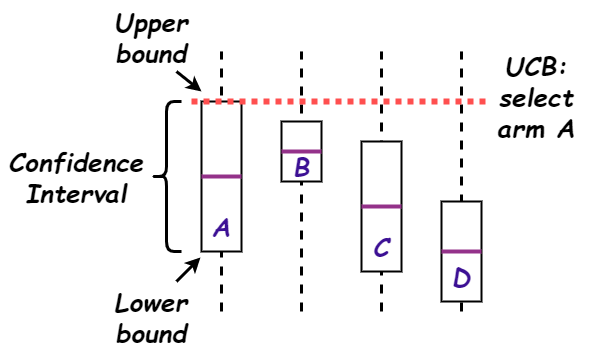
\includegraphics[width=\textwidth]{Images/UCB.png}
\end{exampleBox}

Доверительный интервал можно построить при помощи следующего неравенства:

\begin{theorem}[Неравенство Хёфдинга]
\setcounter{footnote}{1}
Пусть $X_1 \dots X_n$ --- i.i.d выборка из распределения на домене\footnote{мы всегда предполагаем ограниченность наград; для удобства записи будем считать, что диапазон награды --- $[0, 1]$.} $[0, 1]$ с истинным средним $\mu$, $\hat{\mu} \coloneqq \frac{1}{N} \sum_i^N X_i$ --- выборочная оценка среднего. Тогда $\forall u > 0$:
$$\Prob(\mu \ge \hat{\mu} + u) \le e^{-2nu^2}$$
\begin{proof}[Без доказательства]
\end{proof}
% Для произвольного $s$ верен такой переход:
% \begin{align*}
% \Prob(\hat{\mu} \ge \mu + u) &= \Prob(\sum_{i = 1}^n X_i \ge n(\mu + u)) = \Prob(\prod \exp^{s X_i} \ge \exp^{n(\mu + u)}) \le \\
% &\le \frac{\E \prod \exp^{s X_i}}{\exp^{n(\mu + u)}} = \\ 
% &= \left( \frac{\E \exp^{s X}}{\exp^{\mu + u}} \right)^n
% \end{align*}

% Выберем $s$ так, чтобы величина в скобках была как можно меньше, и покажем, что она равна $\exp^{-2u^2}$. Для этого заметим, что для любой реализации $X$ в силу его принадлежности $[0, 1]$ и выпуклости функции $e^x$:
% $$e^{sx} \le (1 - x) e^{s \cdot 0} + x e^{s \cdot 1} = 1 - x + x e^s$$
% Возьмём мат.ожидание слева и справа:
% $$\E e^{sx} = 1 - \mu + \mu e^s = \exp^{\log (1 - \mu + \mu e^s)}$$
% Обозначим $\phi(s) \coloneqq \log (1 - \mu + \mu e^s)$. Разложим её в ряд Тейлора до второго члена с центром в нуле:
% $$\E e^{sx} = \exp^{\phi(0) + s\phi'(0) + \frac{s^2}{2}\phi(\eta)},$$
% где $\eta$ --- некоторая вещественная точка. Ну, $\phi(0) \HM= 0$, посчитаем три производные:
% $$\phi'(s) = \frac{\mu e^s}{1 - \mu + \mu e^s}$$
% $$\phi''(s) = \frac{\mu (1 - \mu) e^s}{(1 - \mu + \mu e^s)^2}$$
% $$\phi'''(s) = \frac{\mu (1 - \mu) (1 - \mu - \mu e^s)}{(1 - \mu + \mu e^s)^3}$$
% Получаем, что $\phi'(0) \HM= \mu$, а $\phi(s'')$ --- вогнутая функция с точкой экстремума в $e^s = \frac{1 - \mu}{\mu}$. Это значит, что
% $$\phi''(\eta) \le \phi''(\frac{1 - \mu}{\mu}) = \frac{(1 - \mu)^2}{4(1 - \mu)^2)} = \frac{1}{4}$$
% Подставляя в:
% $$\E e^{sx} \le \exp^{\mu s + \frac{1}{8}s^2}$$
% Значит,
% $$\Prob(\hat{\mu} \ge \mu + u) \le \left( \exp^{\mu s + \frac{1}{8}s^2 - \mu s - su} \right)^n$$
% Минимизируя $\frac{1}{8}s^2 - su$ по $s$, получаем оптимальное значение $s = 4u$. Подставляя, получаем:
% $$\Prob(\hat{\mu} \ge \mu + u) \le \exp^{-2nu^2}$$
\end{theorem}

Мы можем переформулировать эту теорему в терминах доверительного интервала:

\begin{proposition}
Для любого $\delta$ с вероятностью $1 - \delta$ истинное значение $Q(a)$ не превосходит $Q_k(a) \HM+ U_k(a)$, где:
$$U_k(a) \coloneqq \sqrt{\frac{-\ln \delta}{2n_k(a)}}$$
\begin{proof}
В силу неравенства Хёфдинга:
$$\Prob (Q(a) \ge Q_k(a) + U_k(a)) \le \exp^{-2 n_k(a) U_k(a)^2}$$
Возьмём заданное $\delta$ и прогарантируем, что $\exp^{-2 n_k(a) U_k(a)^2} \HM= \delta$. Разрешая это равенство относительно $U_k(a)$, получаем доказываемое.
\end{proof}
\end{proposition}

В качестве $\delta$ на $k$-ом шаге будем выбирать, например, $\frac{1}{k^c}$, где $c$ --- гиперпараметр. Таким образом, истинное значение будет всё с большей вероятностью оказываться внутри доверительного интервала. Итого в алгоритме UCB предлагается следующая формула выбора действия на очередном $k$-ом шаге:
\begin{equation}\label{UCB}
a_k = \argmax_a \left[ Q_k(a) + c \sqrt{\frac{\log k}{n_k(a)}} \right]
\end{equation}

Получается интерпретируемая формула: числитель $\sqrt{\log k}$ гарантирует, что если некоторое действие давно не выбиралось (счётчик $n_k(a)$ не меняется с увеличением числа итераций $k$), то добавленное слагаемое будет неограниченно расти и в какой-то момент промотивирует попробовать данное действие ещё раз.

%TODO: Теорема Auer, 2002
\begin{theorem}
UCB-алгоритм \eqref{UCB} асимптотически оптимален.
\begin{proof}[Без доказательства]\end{proof}
\end{theorem}

\subsection{Сэмплирование Томпсона}

Мы далее попробуем учить степень нашей неопределённости в знаниях об $Q(a)$, моделируя всё неизвестное распределение $p(r \HM\mid a)$, а не только среднюю награду. Таким образом, мы перейдём к model-based подходу в RL, в котором динамику среды предлагается пытаться учить. В случае с бандитами под динамикой среды подразумеваются распределения награды для каждого автомата $p(r \HM\mid a)$, для чего мы воспользуемся стандартным байесовским подходом.

Введём предположение, что распределения наград $p(r \HM\mid a)$ принадлежат некоторому параметрическому семейству; для каждого автомата заданы значения параметров этого семейства $\theta_a \HM\in \Theta$, и награда генерируется из распределения $p(r \HM\mid \theta_a)$. Однако, истинные значения $\theta_a$ нам неизвестны.

Вместо оценки максимального правдоподобия на $\theta_a$ будем делать \emph{байесовский вывод}. Зададимся некоторым \emph{априорным распределением} (<<прайором>>) $p(\theta_a)$ для каждого действия $a$ (сюда мы можем в том числе положить какую-то дополнительную априорную информацию о том, какие автоматы заведомо лучше), и после очередного эпизода игры с автоматом $a$ с исходом $r_k$ будем обновлять распределение над $\theta_a$ по формуле Байеса на \emph{апостериорное распределение}:
\begin{equation*}
p(\theta_a) \leftarrow p(\theta_a \mid r_k) \propto p(r_k \mid \theta_a)p(\theta_a)
\end{equation*}

Таким образом мы аккумулируем всю информацию о значениях $\theta_a$, полученную из всех имеющихся сэмплов награды и исходного априорного распределения. Средний выигрыш из автомата $a$, соответственно равный $\E p(r \mid \theta_a)$, теперь для нас будет являться случайной величиной, поскольку $\theta_a$ --- случайное, с распределением $p(\theta_a)$.

\begin{example}[Bernoulli-бандиты]
Положим, что автоматы выдают только награду 0 или 1, то есть что истинное распределение есть распределение Бернулли с вероятностью $\theta_a$:
$$p(r \mid a) \coloneqq \operatorname{Bernoulli}(r \mid \theta_a) = \theta_a^{\mathbb{I}[r = 1]}(1 - \theta_a)^{\mathbb{I}[r = 0]} = \theta_a^{r}(1 - \theta_a)^{1 - r}$$

Априорное распределение зададим при помощи \href{https://en.wikipedia.org/wiki/Beta_distribution}{Бета-распределения}\footnote[1]{это распределение является \emph{сопряжённым} (conjugate) к Бернулли, что означает, что после применения формулы Байеса наше распределение останется в этом же семействе распределений.} распределения, а то есть:
$$p(\theta_a) \coloneqq \operatorname{Beta}(\theta_a \mid \alpha, \beta) \propto \theta_a^{\alpha - 1}(1 - \theta_a)^{\beta - 1}$$
где $\alpha$ и $\beta$ --- некоторые параметры (свои для каждого автомата $a$). Мы можем обновлять эти знания при помощи новых сэмплов $r_k \HM\sim p(r \mid a)$, проводя байесовский вывод. Применяем формулу Байеса:
$$p(\theta_a \mid r) \propto \underbrace{\theta_a^{r_k}(1 - \theta_a)^{1 - r_k}}_{p(r_k \mid \theta_a)}\underbrace{\theta_a^{\alpha - 1}(1 - \theta_a)^{\alpha - 1}}_{p(\theta_a)} = \operatorname{Beta}(\theta_a \mid \alpha + r_k, \beta + 1 - r_k)$$
Таким образом, для обновления параметров $\alpha, \beta$ достаточно увеличить $\alpha$ на $r_k$, а $\beta$ --- на $1 - r_k$.

При заданном $\theta_a$ мы можем посчитать среднее значение выигрыша, ценность автомата $a$: для случайной Бернуллиевской величины с параметром $\theta_a$ среднее, сообственно, совпадает с $\theta_a$: 
$$\hat{Q}(a) = \E p(r \mid \theta_a) = \theta_a$$

Тогда, имея $\alpha$ и $\beta$, мы всегда можем посчитать мат.ожидание выигрыша в нашей модели:
$$\E_{\theta_a} \hat{Q}(a) = \E_{\operatorname{Beta}(\theta_a \mid \alpha, \beta)} \theta_a = \frac{\alpha}{\alpha + \beta}$$
Как видно, оно не отличается от Монте-Карло оценки Q-функции: $\alpha$ имеет смысл <<успехов>>, когда Бернулливская величина выкинула нам единичку, а $\beta$ --- число неуспехов, нулей, и формула обновления этих параметров в точности соответствует подсчёту этих счётчиков; при выборе прайора $\alpha \HM= \beta \HM= 0$ мы получим в формуле мат.ожидания отношение числа успехов к общему числу попыток. 

Однако теперь у нас есть не только оценка среднего значения $\theta_a$, но и вероятности для каждого его возможного значения. На рисунке далее приведены $p(\theta_a)$ для разных значений $\alpha$ (<<успехов>>) и $\beta$ (<<неудач>>) при прайоре $\alpha \HM= \beta \HM= 1$:

\begin{center}
    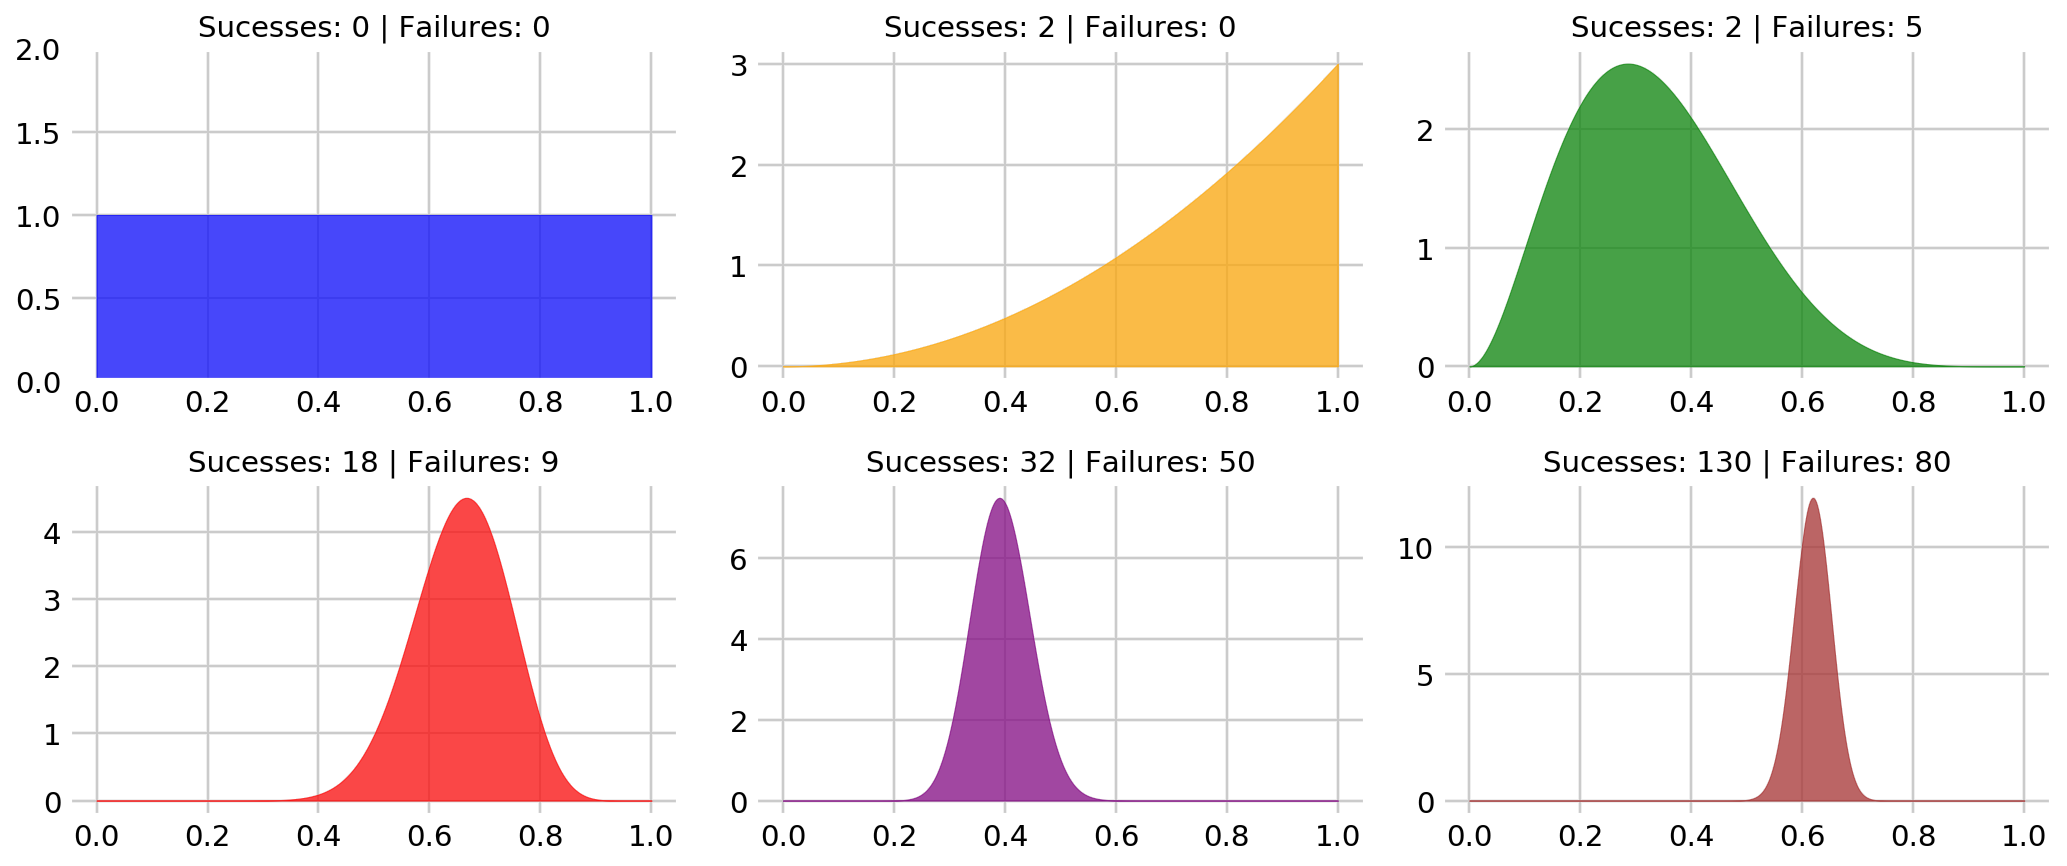
\includegraphics[width=\textwidth]{Images/TS}
\end{center}
\end{example}

Как пользоваться полученным апостериорным распределением? Мы можем реализовать идею, которая называется \emph{probability matching}. Согласно текущим $p(\theta_a)$ жадный выбор действия имеет вид
$$a \HM\coloneqq \argmax_a \E_{\theta_a \sim p(\theta_a)} \E p(r \mid \theta_a),$$
но теперь в нашей модели есть некоторая вероятность и того, что такое действие на самом деле неоптимально. Мы можем посчитать эту вероятность, то есть с учётом распределений $\theta_a$ посчитать вероятность, что хотя бы для одного другого автомата $\hat{a} \ne a$
$$\E p(r \mid \theta_{\hat{a}}) > \E p(r \mid \theta_{a}),$$
и посмотреть, с какой вероятностью мы ошибёмся. Аналогично можно для любого действия посчитать вероятность того, что на самом деле оптимальным является оно. Предлагается ровно с такими вероятностями, собственно, и выбирать автомат на очередном шаге.

\begin{definition}
\emph{Сэмплированием Томпсона} (Thompson Sampling) называется процедура, при котором на $k$-ом шаге при решении задачи многоруких бандитов действие $a$ выбирается с вероятностью того, что оно оптимально в рамках выученных моделей $p(\theta_a)$:
$$\pi(a) \coloneqq \Prob \left( \E p(r \mid \theta_a) = \max_{\hat{a}} \E p(r \mid \theta_{\hat{a}}) \right)$$
\end{definition}

Посчитать такие вероятности может быть нетривиально, зато легко из такого распределения сэмплировать (отсюда название\footnote{забавный факт: Томпсон вообще первый рассмотрел задачу многоруких бандитов, и в качестве эвристического решения предложил сэмплировать из моделей и брать аргмаксимум из сэмплов. То есть, можно сказать, сэмплирование Томпсона было первым придуманным способом решения задачи. А позже через почти век выяснилось, что это решение асимптотически оптимально.}). Действительно: просто для каждого действия $a$ засэмплируем $\theta_a$ из текущего $p(\theta_a)$, и, соответственно, выберем автомат с наибольшим мат.ожиданием согласно выпавшим $\theta_a$. 

\begin{example}
Допустим, мы храним информацию о распределениях $p(r \mid a)$ в Бета-распределениях, как в предыдущем примере. Для всех действий сэмплируем $\theta_a \sim \operatorname{Beta}(\theta_a \mid \alpha_a, \beta_a)$ при выученных параметрах $\alpha_a, \beta_a$, и считаем мат.ожидание соответствующего распределения Бернулли при выпавших параметрах $\theta_a$ --- для распределения Бернулли среднее совпадает с $\theta_a$ в точности. Таким образом, мы выберем автомат, для которого выпало наибольшее значение сэмпла $\theta_a$.
\end{example}

Идея в том, что для автоматов, которые мы пробовали часто, дисперсия апостериорного распределения будет маленькой и сэмпл почти всегда будет в точности равен текущей оценке Q-функции. Для автоматов, которые мы пробовали редко в силу маленького реварда, дисперсия будет большая и иногда сэмплы будут оказываться лучше текущего самого хорошего автомата, что заставит нас поэксплорить данный автомат ещё.

\begin{algorithm}{Beta-Bernoulli Бандит с сэмплированием Топмсона}
\textbf{Гиперпараметры:} $\alpha, \beta$ --- параметры прайора.

\vspace{0.3cm}
Обнулить счётчики $\alpha_0(a) \coloneqq \alpha, \beta_0(a) \coloneqq \beta$ \\
\textbf{На очередном шаге $k$:}
\begin{enumerate}
    \item сгенерировать $\theta_a \sim \operatorname{Beta}(\alpha_k(a), \beta_k(a))$
    \item выбрать $a_k \coloneqq \argmax\limits_{a} \theta_a$
    \item пронаблюдать $r_k \in \{0, 1\}$
    \item обновить счётчик $\alpha_k(a) \coloneqq \alpha_{k-1}(a) + [a_k = a][r_k = 1]$
    \item обновить счётчик $\beta_k(a) \coloneqq \beta_{k-1}(a) + [a_k = a][r_k = 0]$
\end{enumerate}
\end{algorithm}

\begin{theorem}
Сэмплирование Томпсона асимптотически оптимально.
\begin{proof}[Без доказательства]\end{proof}
\end{theorem}

\begin{example}
Поиграться с визуализацией этого алгоритма можно \href{https://learnforeverlearn.com/bandits/}{здесь}.
\end{example}

% TODO: пример с графом дорог

% TODO: Bayesian RL